\section{Prototyping}

\paragraph{A prototype is a useful design tool for testing concepts, clarifying requirements, and starting user interaction and feedback.
Prototyping methods can be categorized by fidelity—ranging from low-fidelity sketches to high-fidelity digital mockup.}


\subsection{Prototype methods}
\paragraph{We use Evolutionary prototyping to continuously update our prototypes.Part of the prototyping process involves dealing with feedback and subsequent revisions. It helps designers test and retest their ideas over and over again. The faster designers are able to test their design concepts and make improvements, the faster they can get to a satisfactory final version. In addition, our team uses Agile development methodologies in prototyping. Agile increases flexibility, collaboration, and rapid feedback cycles to create product prototypes in rapid iterations with continuous ones after collecting feedback and guided ones.}


\subsection{Low-fidelity prototypes}

\item \textbf{Sketches}
\paragraph{We used FigJam for the sketch concept, which allowed us to do a full online brainstorm. we started out with a card format, where the top right side displays the filter and the bottom side displays the rotation of the three icon styles, and the top left and bottom left side have the branding icon and the cookie component, which made the whole page more cluttered. This made the whole page more complicated, so we updated it so that the filter, radius range are on the right as a whole dashboard, and the branding icon is also moved to the dashboard, so that users can better remember our brand.}


\begin{figure}[h]
    \centering
    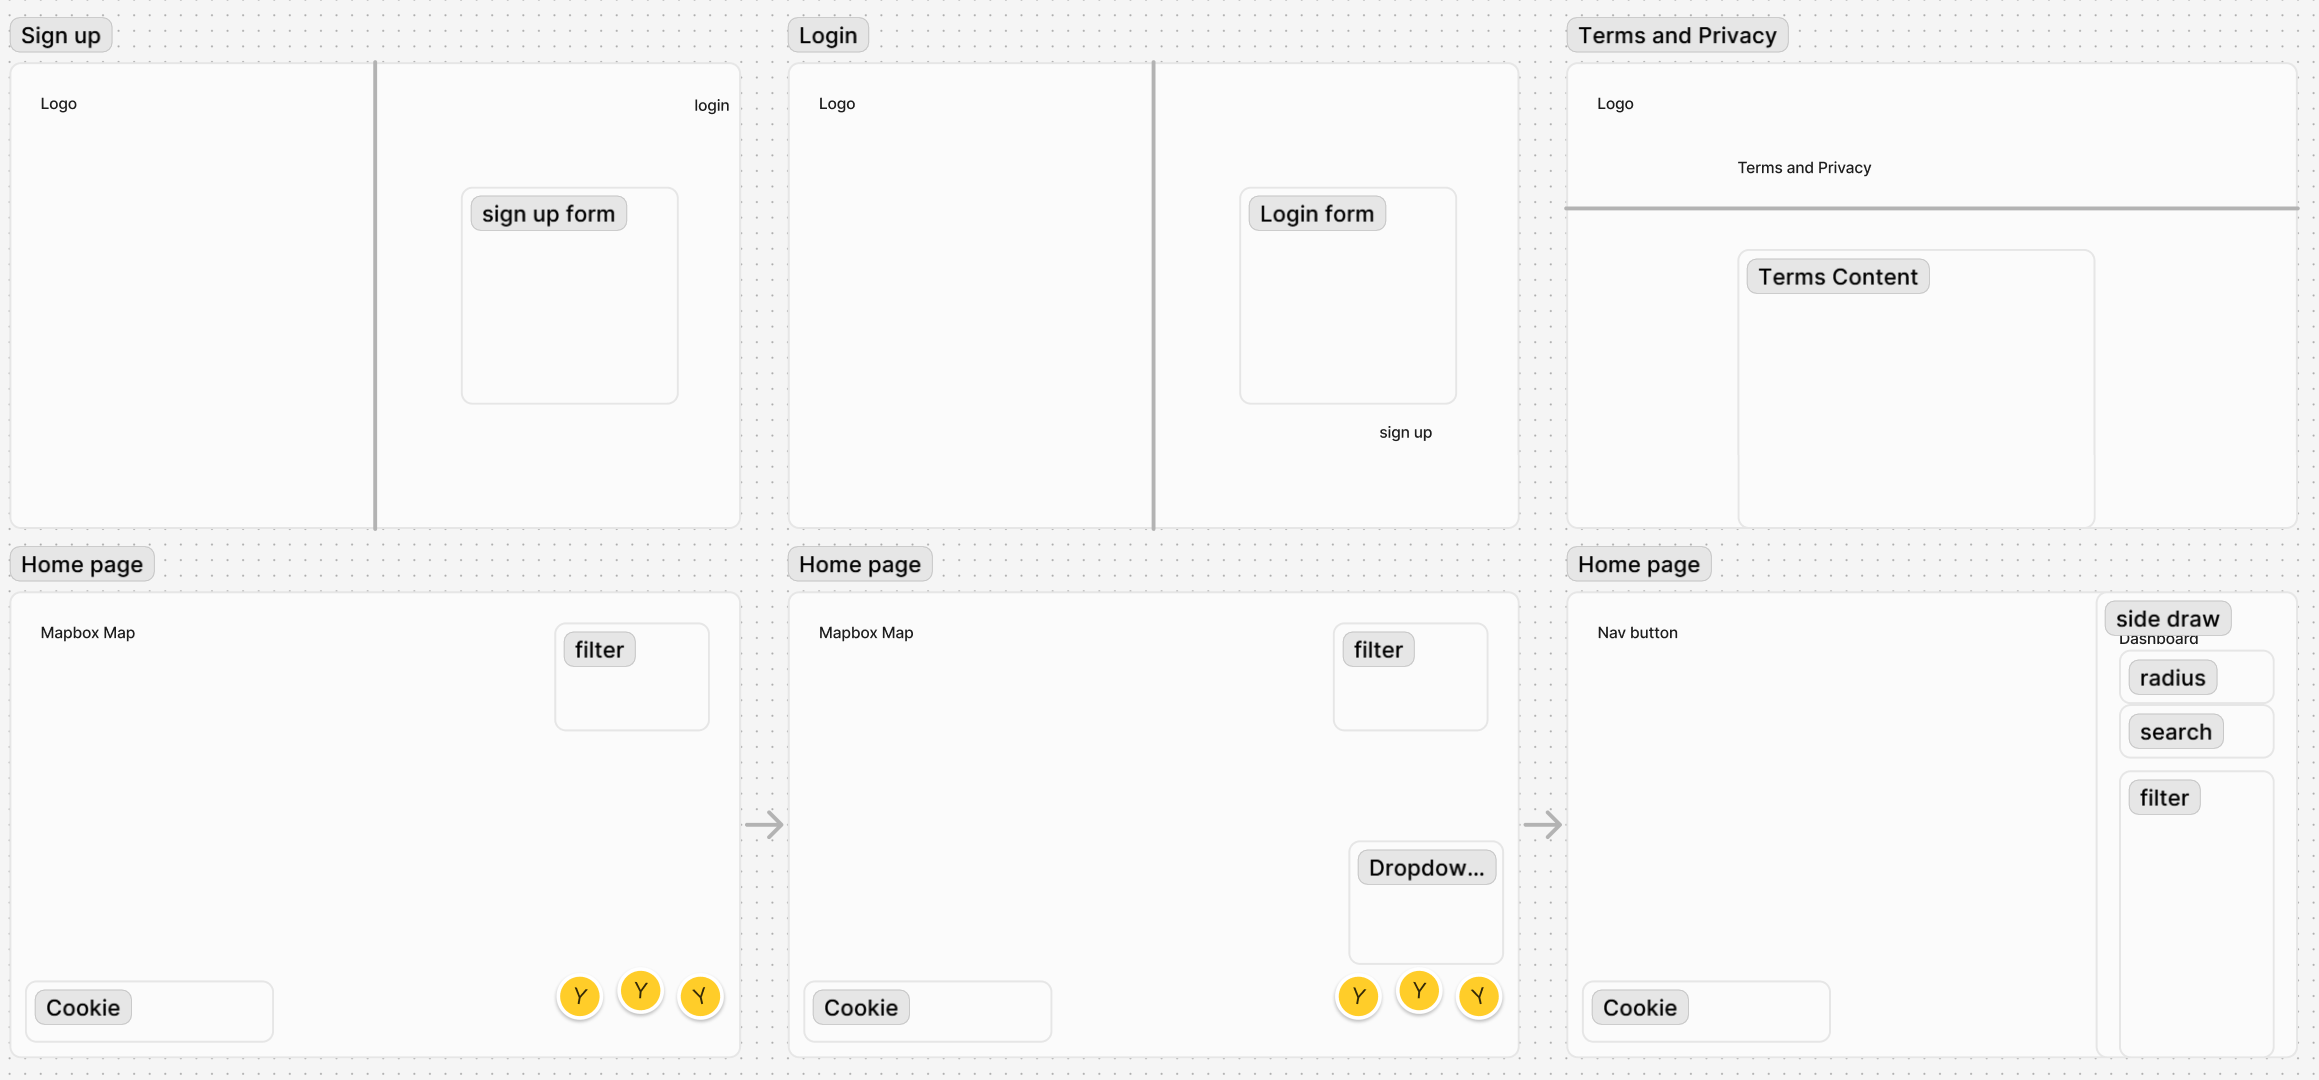
\includegraphics[width=0.48\textwidth]{images/sketch.jpg}
    \caption{Evolution of interface design from initial card-based layout to consolidated dashboard approach}
    \label{fig:prototype-evolution}
\end{figure}

\paragraph{This evolution in our design approach demonstrates the value of iterative prototyping in achieving a balance between functionality and visual clarity. The final layout creates a more focused user experience while maintaining all essential features in an intuitive, accessible format.}

\item \textbf{Wireframe}
\paragraph{Wireframe as a low-fidelity tool, unlike sketches, wireframes show the structure of an interface design, but often lack detail or colour. We also made wireframes of individual pages to build on, such as the home page and the login/signup page in Figure~\ref{fig:wireframe-home} and Figure~\ref{fig:wireframe-signup}, which lay out the structure of the prototype.}
\begin{figure}[h]
    \centering
    \begin{minipage}{0.48\textwidth}
        \centering
        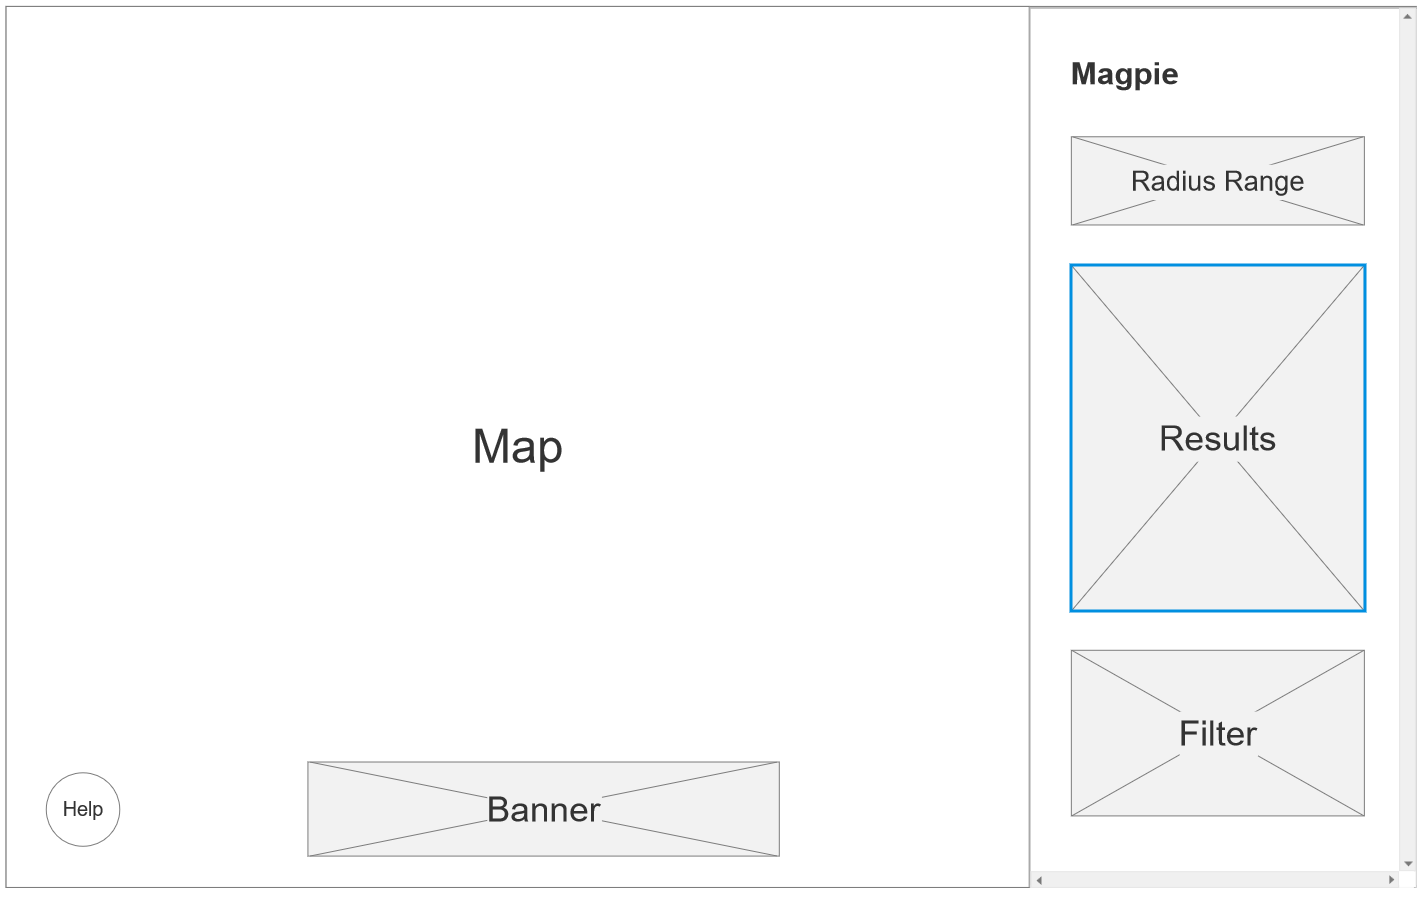
\includegraphics[width=\textwidth]{images/wireframe-home.jpg}
        \caption{Wireframe-home}
        \label{fig:wireframe-home}
    \end{minipage}
    \hfill
    \begin{minipage}{0.48\textwidth}
        \centering
        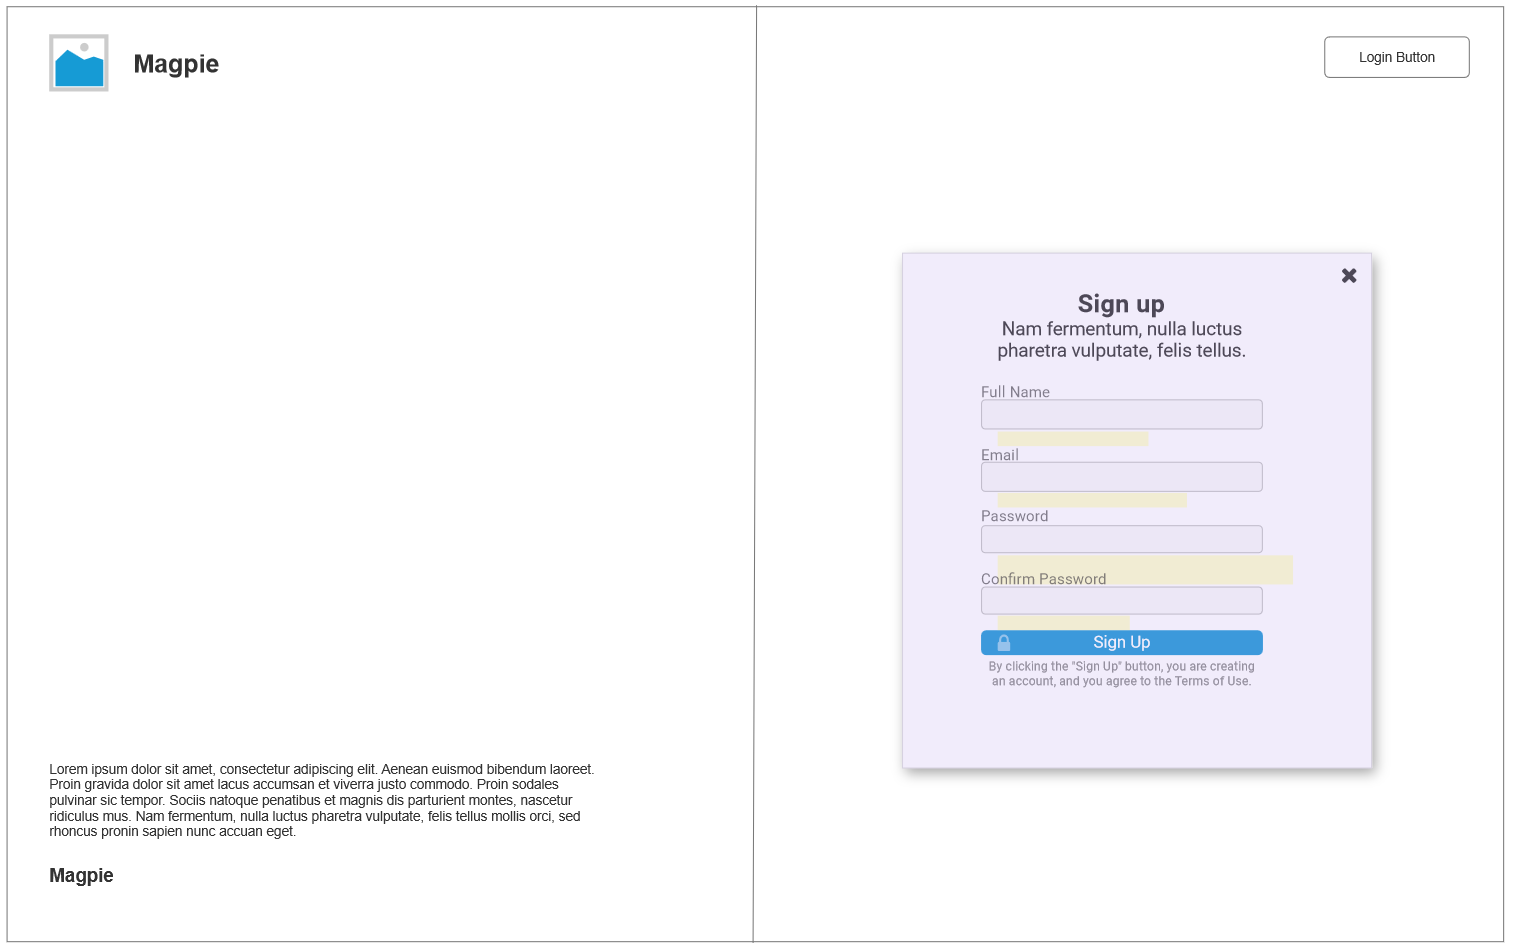
\includegraphics[width=\textwidth]{images/wireframe-signup.jpg}
        \caption{Wireframe-login/signup}
        \label{fig:wireframe-signup}
    \end{minipage}
\end{figure}

\subsection{Medium and High Fidelity Prototyping}
\paragraph{Medium-fidelity prototypes offer more detail, serving as a transitional phase between initial ideas and advanced user testing.}

\paragraph{As we move from medium to high fidelity, the prototypes become more refined and detailed, incorporating more realistic interactions and visual elements. This transition allows us to test more specific aspects of the user experience and gather more precise feedback.}

\paragraph{High-fidelity prototypes closely resemble the final product in both form and function.}

\paragraph{The first version of the prototype design is very similar to the sketch and wireframe designs, but it did not take into account the needs and experiences of the users, so it needs to be iterated. The card-based design makes the entire home screen very cluttered and scattered, and the login/signup page adopts the original shadcn style, which needs to be customized and improved.}

\subsection{User Interface Iteration}
Iteration 1:

第一版的prototype设计和sketch设计和wireframe设计很像, 但是没有考虑到用户的需求和体验, 所以需要进行迭代.卡片式设计使得整个home屏幕很乱很分散,login/signup页面采用了原版的shadcn样式需要进行定制化改进。


